%----------------------------------------------------------------------------------------
%	CHAPTER - INTRODUCTUION
%----------------------------------------------------------------------------------------

\chapter{Introduction} % Main chapter title

\label{ChapterIntroduction} % Change X to a consecutive number; for referencing this chapter elsewhere, use \ref{ChapterX}

%----------------------------------------------------------------------------------------
%	SECTION 1
%----------------------------------------------------------------------------------------

\section{Introduction}

With the public release of the Oculus Rift in March 2016 \citep{Oculus2016} and the HTC Vive in April 2016 \citep{Htcvive2016}, virtual reality has arrived at the consumer level and is all over the news. Although we only see the first iteration of consumer products, \cite{Gartner2015} predicts that within the next five to ten years, virtual reality will achieve mainstream adoption and enter the so called "Plateau of Producitivity". Gesture Control is even a bit ahead of VR and its mainstream adoption is already expected in the next two to five years \citep{Gartner2015}.

The focus of this master thesis is on the possibilities of enhanced user interaction with virtual reality by utilizing not only hand gestures, but making use of the additional sensor information of gesture controllers and 360° motion tracking.

In the following subchapters, more background information about the topic is given as well as the definition of the problem statement. Based on this, the thesis statement is proposed and research questions are derived from. Following this, the delineations and limitations are presented before this chapter is closed with the structure of the thesis and a brief overview of the chapters and their corelations.


%----------------------------------------------------------------------------------------
%	SECTION 2
%----------------------------------------------------------------------------------------

\section{Background}

blub
% TODO: COMPLETE


(Figure \ref{fig:hypecycle}). This means that if Gartner is to be beliefed, Virtual Reality has the phase of over-excitement and unrealistic expectations already behind it and VR is close to the point where it is widely understood by the general public. A bit further than VR itself is Gesture Control that according to \cite{Gartner2015} will already reach mainstream adoption in the next two to five years.
\begin{figure}[h]
	\begin{center}
		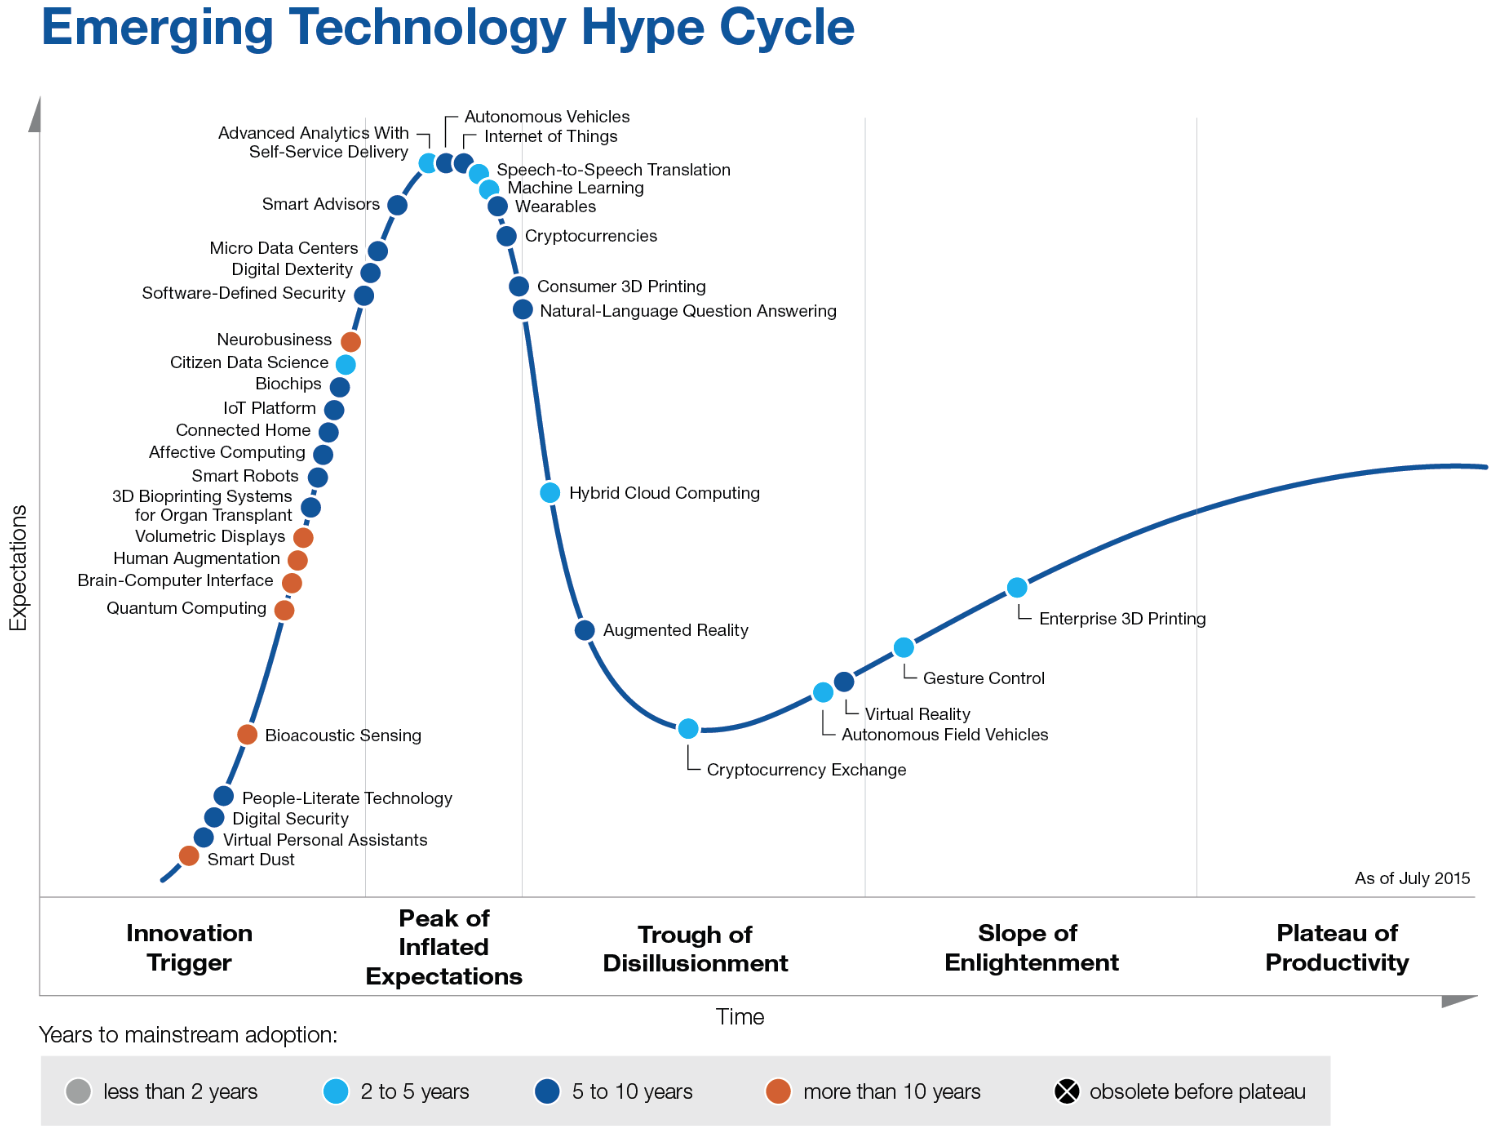
\includegraphics[width=14cm]{03_Figures/03_Gartner/Gartner_EmergingTech2015.png}
		\caption[Emerging Technology Hype Cycle]{Emerging Technology Hype Cycle \citep{Gartner2015b}}
		\label{fig:hypecycle}
	\end{center}
\end{figure}



blub
\cite{Safrudin2015}
blub

%----------------------------------------------------------------------------------------
%	SECTION 3
%----------------------------------------------------------------------------------------

\section{Problem Statement}

blub
% TODO: COMPLETE


%----------------------------------------------------------------------------------------
%	SECTION 4
%----------------------------------------------------------------------------------------

\section{Thesis Statement}

The tesis statement is as follows: \newline
\textit{The interaction with multidimensional data in virtual reality can be enhanced by utilizing gesture controllers and 360° motion tracking.}


%----------------------------------------------------------------------------------------
%	SECTION 5
%----------------------------------------------------------------------------------------

\section{Research question}

To adress the problem statement, research questions are used to break down the research into smaller parts that can be examined individually and allow a view at the nature of the problem from different perspectives.
In this chapter, the \gls{mrq} as well as the \glspl{srq} are formulated. \newline
The main resarch question, derived from the thesis statement, is:
\begin{framed}
	\textit{Can the interaction with multidimensional data in virtual reality be enhanced by utilizing gesture controllers and 360° motion tracking?}
\end{framed} \label{MRQ}
From the MRQ, the SRQs can be derived and are defined as follows:
\begin{framed}
	\textit{SRQ 1: Which ways of interaction with multi-dimensional exist and what are their strengths and weaknesses?}
\end{framed} \label{SRQ1}
\begin{framed}
	\textit{SRQ 2: tbd}
\end{framed} \label{SRQ2}
\begin{framed}
	\textit{SRQ 3: How can the retrieved sensor information be used to enhance existing interaction patterns with multidimensional data?}
\end{framed} \label{SRQ3}
 

%----------------------------------------------------------------------------------------
%	SECTION 6
%----------------------------------------------------------------------------------------

\section{Research Objective}

The research objective of this master thesis is to enhance the interaction with data in virtual reality by proposing the utilization of sensor information from gesture controllers and 360° motion tracking.\newline
This objective will be adressed by first conducting a literature review on the research that has already been done in this field. Based on this a possible prototype will be designed and implemented that will make use if the to be proposed interaction patterns. This also acts as a verification that the interaction patterns indeed are feasible for the currently available technology.


%----------------------------------------------------------------------------------------
%	SECTION 7
%----------------------------------------------------------------------------------------

% \section{Short Overview}


%----------------------------------------------------------------------------------------
%	SECTION 8
%----------------------------------------------------------------------------------------

\section{Delineations and Limitations}

In this thesis, the focus lies on interaction possibilites with gesture controllers and 360° motion tracking. Other means of input data such as from speech recongition is not part of the research.
In regards of the design and implementation of the prototype, the artefact will be implemented in Unity3D 5.4 with the SteamVR framework. The hardware in scope for the verification is the HTC Vive since it currently is the only consumer product with the  technical capabilities of gesture controllers and 360° motion tracking. Although focusing on the HTC Vive, due to the SteamVR framework functionality (Figure \ref{fig:steamvr}), the reuse of the research for other hardware should be possible in the future. \newline
Furthermore, with the design and development of a prototype, this thesis focuses more on the technical feasibility than the socioligal aspects of usability, user expercience, or productivity measurements. 
\begin{figure}[h]
	\begin{center}
		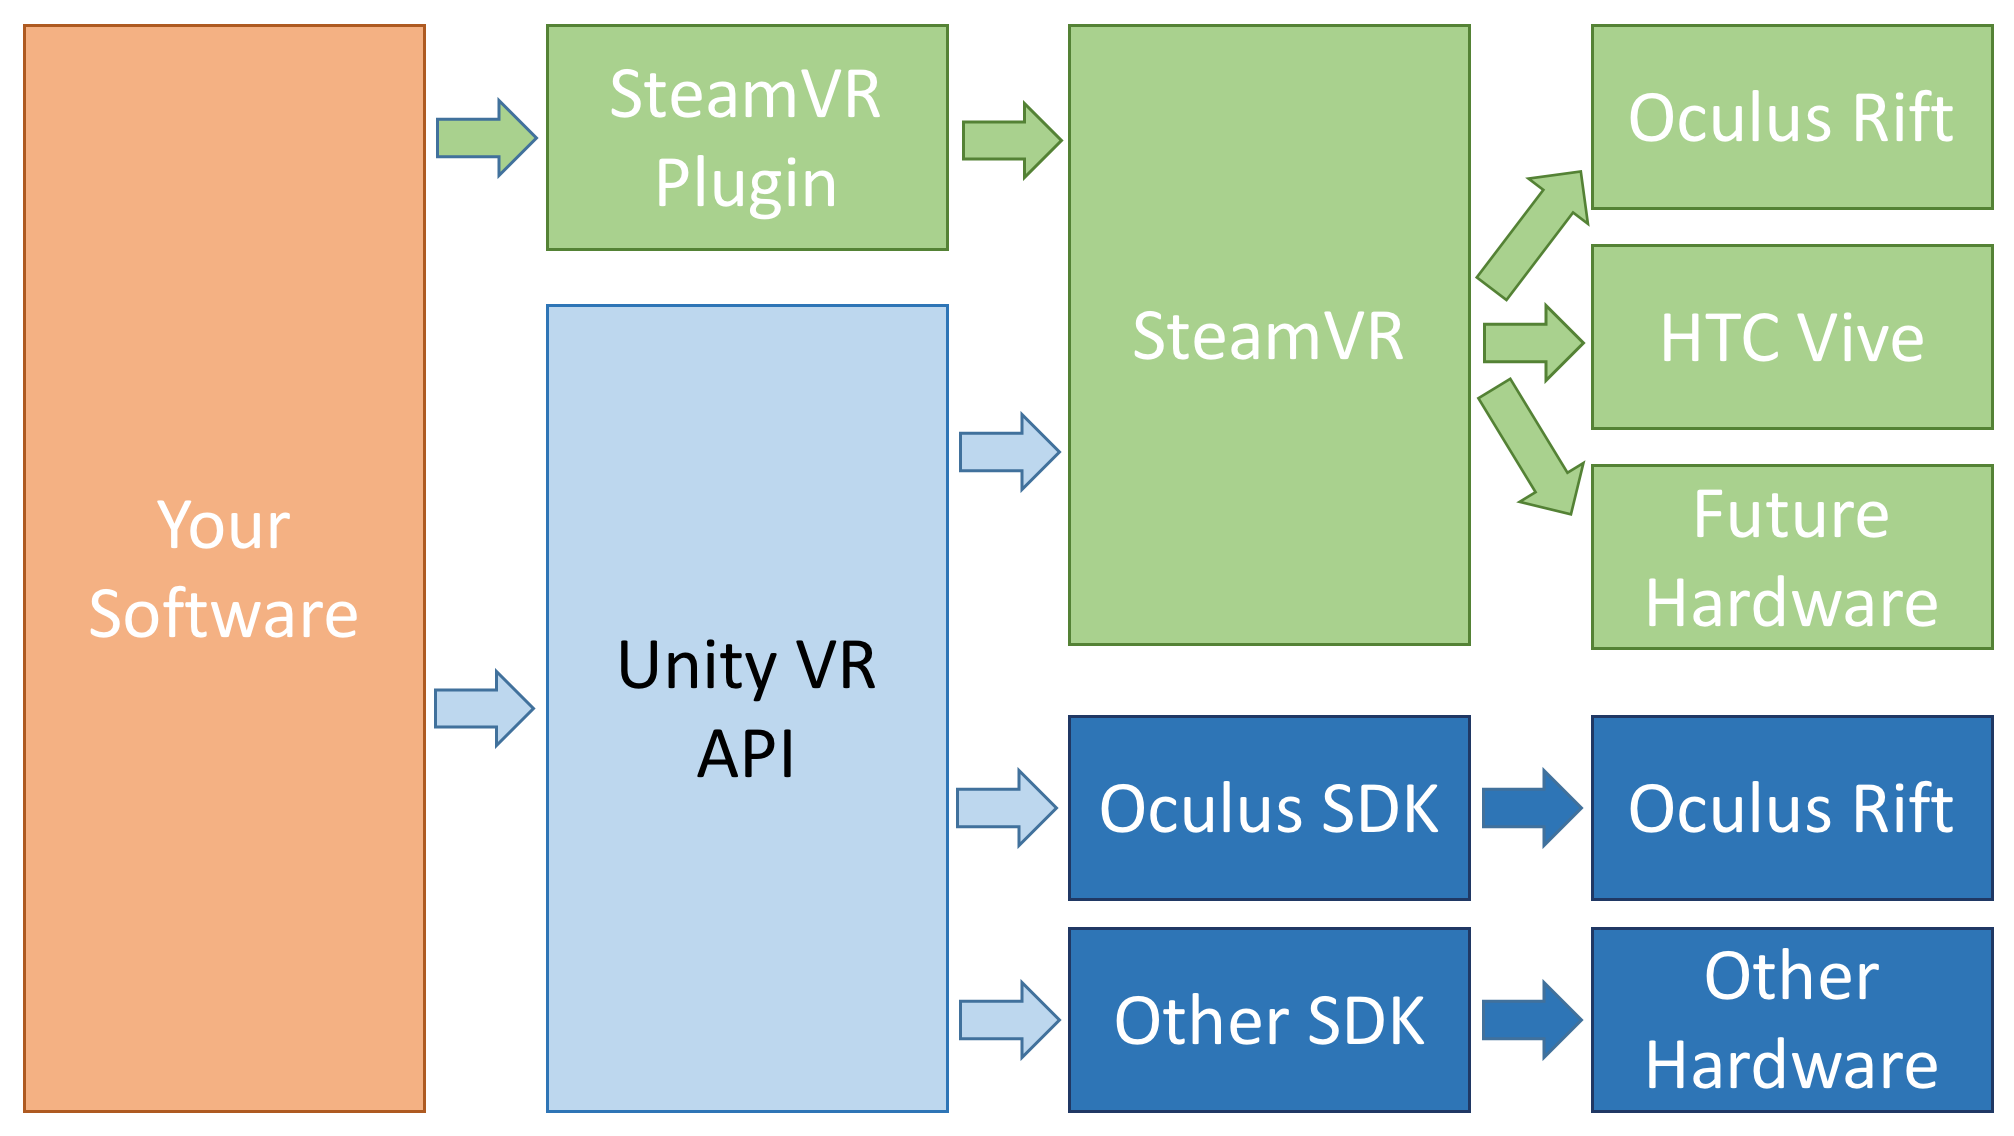
\includegraphics[width=14cm]{03_Figures/04_Valve/OpenVR_SteamVR.png}
		\caption[Steam VR Unity Plugin]{Steam VR Unity Plugin (adopted from \cite{Valve2016})}
		\label{fig:steamvr}
	\end{center}
\end{figure}


%----------------------------------------------------------------------------------------
%	SECTION 9
%----------------------------------------------------------------------------------------

% \section{Underlying Assumptions}


%----------------------------------------------------------------------------------------
%	SECTION 10
%----------------------------------------------------------------------------------------

% \section{Definition of terms and concepts}


%----------------------------------------------------------------------------------------
%	SECTION 11
%----------------------------------------------------------------------------------------

% \section{Significance}


%-----------------------------------
%	SUBSECTION 1
%-----------------------------------

% \subsection{Theoretical}


%-----------------------------------
%	SUBSECTION 2
%-----------------------------------

% \subsection{Practical}


%----------------------------------------------------------------------------------------
%	SECTION 12
%----------------------------------------------------------------------------------------

\section{Thesis structure and brief chapter overviews}

The thesis map on Figure \ref{thesismap} shows the structure of this aper and the relations of the individual chapters. \newline
In chapter \ref{ChapterIntroduction}, an introduction on the topic and the research problem is given. From this the thesis statement, research questions and the research objectives are derived. Following in Chapter \ref{ChapterLiteratureReview} comes the literature review of...
% TODO: COMPLETE 
The research methodology follows in chapter \ref{Research Method} where the philosophy, approach and strategy are described.

%----------------------------------------------------------------------------------------
%	SECTION 13
%----------------------------------------------------------------------------------------

% \section{Any other institutional requirement not covered here}



